\documentclass[conference,letterpaper]{IEEEtran}
\usepackage[T1]{fontenc}
\usepackage{booktabs,tabularx,graphicx,tikz}
\usetikzlibrary{arrows.meta,positioning}
\usepackage[hidelinks]{hyperref}
\graphicspath{{../../../../../KB/Poppy_KB_v0.6.1/case-6/}}
\title{Ppopy: Architecture Design and Partial Implementation}
\author{\IEEEauthorblockN{Doyeong Koo, Takgeon Kang, Geonil Won}
\IEEEauthorblockA{Team CosMate, CSE 406 Software Engineering\\Hanyang University}}
\begin{document}
\maketitle
\begin{abstract}
This report continues the Phase 2 A/B specification with an architecture, a source map, and step-by-step use cases for Ppopy. The implemented iPhone workflow connects product identification, versioned ingredient data, morning and evening routines, adaptive questions, and saved results. The authorized smart mirror and timing-based delivery remain integration targets. The report records which behaviors were exercised in local tests, on the public API, and on an iPhone.
\end{abstract}
\begin{IEEEkeywords}
skincare routine, knowledge base, adaptive question selection, iOS
\end{IEEEkeywords}
\setcounter{section}{4}
\section{Architecture Design \& Implementation (Partial)}

\subsection{Overall Architecture}
The iOS client submits the confirmed routine and answers to the public HTTP API. The backend checks account access and consent, then passes confirmed observations to the decision engine. The engine evaluates relevant cleansing, moisturizing, and sun-protection rules and exceptions. Adaptive feature acquisition (AFA) chooses a question when a plausible answer changes a proposed action. When no useful question remains, the app shows what to keep, what to adjust, and what remains uncertain. Figure~\ref{fig:architecture} shows the implemented flow and the planned mirror integration.

\begin{figure*}[!t]
\centering
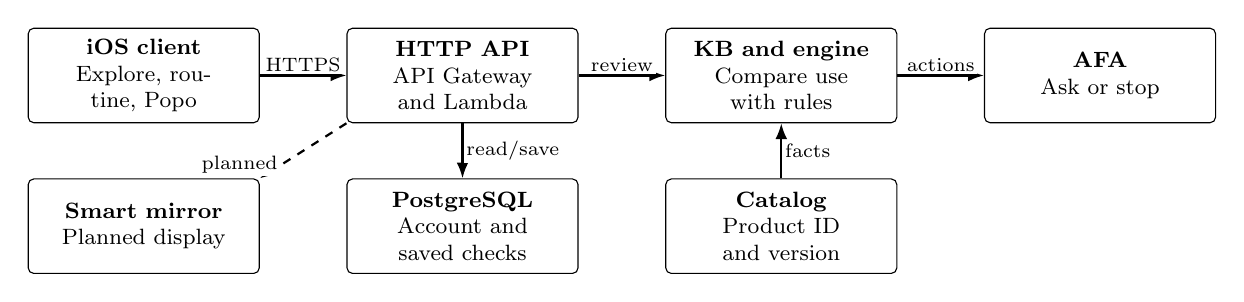
\begin{tikzpicture}[node distance=7mm and 11mm, box/.style={draw,rounded corners=2pt,align=center,text width=27mm,minimum height=12mm,font=\footnotesize}, edge/.style={-{Latex[length=2mm]},thick}, lab/.style={font=\scriptsize,fill=white,inner sep=1pt}]
\node[box] (app) {\textbf{iOS client}\\Explore, routine, Popo};
\node[box,right=of app] (api) {\textbf{HTTP API}\\API Gateway and Lambda};
\node[box,right=of api] (kb) {\textbf{KB and engine}\\Compare use with rules};
\node[box,right=of kb] (afa) {\textbf{AFA}\\Ask or stop};
\node[box,below=of app] (mirror) {\textbf{Smart mirror}\\Planned display};
\node[box,below=of api] (db) {\textbf{PostgreSQL}\\Account and saved checks};
\node[box,below=of kb] (cat) {\textbf{Catalog}\\Product ID and version};
\draw[edge] (app) -- node[lab,above]{HTTPS} (api);
\draw[edge] (api) -- node[lab,above]{review} (kb);
\draw[edge] (kb) -- node[lab,above]{actions} (afa);
\draw[edge] (api) -- node[lab,right]{read/save} (db);
\draw[edge] (cat) -- node[lab,right]{facts} (kb);
\draw[edge,dashed] (api.south west) -- node[lab,left,near end]{planned} (mirror.north east);
\end{tikzpicture}
\caption{Ppopy components. The app receives either the selected question or the guidance through the HTTP API. The dashed edge shows the planned authorized display path.}
\label{fig:architecture}
\end{figure*}

\subsection{Directory Organization}
Table~\ref{tab:source} identifies representative entry points. The first five rows are in the public course repository. The last three describe app and backend modules in the private project so reviewers can trace the architecture without operating credentials or member data.

\begin{table}[!t]
\caption{Representative Code and Evidence Locations}
\label{tab:source}
\centering\footnotesize
\setlength{\tabcolsep}{4pt}
\begin{tabularx}{\columnwidth}{@{}>{\raggedright\arraybackslash}p{.26\columnwidth}>{\raggedright\arraybackslash}X>{\raggedright\arraybackslash}X@{}}
\toprule
Directory & Representative file & Module or purpose \\
\midrule
\path{KB/Poppy_KB_v0.6.1/} & \path{sunscreen_removal_review.json} & Versioned sunscreen-removal rule \\
\path{skin_engine/kb_preview/} & \path{__main__.py} & Local preview entry point \\
\path{tests/} & \path{test_kb_preview_current_spec.py} & Current-spec checks and historical audit \\
\path{tools/} & \path{verify_source_manifest.py} & Public snapshot integrity \\
\path{docs/} & \path{verification.md} & Reproduction commands and known gaps \\
\path{frontend/src/} & \path{MirayExplore.tsx}, \path{MemberKbPanel.tsx} & Product and routine-review screens \\
\path{skin_engine/kb_preview/} & \path{member_afa.py} & Member question selection and revision \\
\path{db/} & Versioned SQL migrations & PostgreSQL storage and access contracts \\
\bottomrule
\end{tabularx}
\end{table}

\subsection{iOS Client and Catalog (R2--R3)}
The React/TypeScript interface runs in a Capacitor iOS shell. The Explore component supports product name, brand, and photo input. A bundled catalog lets the app display exact brand matches promptly. The app merges returned candidates by product ID. The catalog links ingredient labels and routine entries by product ID and version. Missing or conflicting labels keep the product searchable and suspend ingredient-based judgments that depend on the missing evidence. The inventory holds owned products; the morning and evening routine records identify which items the user actually uses.

\subsection{Knowledge Base and AFA (R4--R6)}
The Python decision engine reuses the reviewed KB and explicit exceptions. It evaluates product and use facts before suggesting an action. AFA compares candidate outcomes across possible answers. It stops when further answers would leave actionable guidance unchanged. An edited answer invalidates dependent questions and guidance, and the engine evaluates the affected decisions again. Evidence from one sunscreen version does not automatically apply to another version or cleanser combination.

\subsection{Public API and Records (R1, R7, R10)}
API Gateway invokes the versioned Python Lambda. The app saves an explicit checkpoint and can reopen its associated result. Existing sessions and stored results retain their recorded semantics. On November 20, the combined candidate was deployed and its signed app installed and launched on an iPhone 13 Pro. The deployment returned the expected unauthenticated response on four direct probes and four public probes. Authenticated behaviors are covered by local test evidence and require a separate device pass on the combined candidate.

\subsection{Mirror Delivery (R8--R9)}
Submission B specifies one authorized, output-only mirror. The proposed path estimates a routine start from confirmed prior use, evaluates the latest guidance, checks display authorization, and expires stale output. Pairing, proactive delivery, and physical display acknowledgement are pending for this implementation milestone.

\section{Use Cases}

\subsection{Find Products and Read Matched Ingredients (R2, Q2)}
\begin{enumerate}
\item Open Explore and enter \emph{Senka} as the brand.
\item Open the standalone Perfect Whip Facial Wash result and inspect its ingredient list.
\item Search for Rovectin Aqua Deep Cleansing Water 400 mL and open its details.
\item Check that the Rovectin label shows all 30 shared ingredients for the same product version. Two matched sources differ in ordering; the list is displayed without using it as evidence of concentration rank.
\end{enumerate}
The candidate tests cover 1,977 catalog product and routine bindings and five ingredient-evidence states. The combined candidate's on-device brand and ingredient checks are pending.

\subsection{Revise, Save, and Reopen a Review (R3--R7, Q3)}
\begin{enumerate}
\item Open Routine Check, confirm the morning and evening products, and select the recent-breakout concern.
\item In the synthetic case, confirm the general-care branch and answer that the recent change is unknown. Answer yes if the next question asks about repeated rubbing.
\item Edit the earlier answer to indicate that none of the listed changes applies. Check that the dependent rubbing question and guidance disappear.
\item Save the review, reopen it from Saved Checks, and compare the reopened guidance with the revised result. Open a previously saved check to verify that it remains readable.
\end{enumerate}
A local browser integration test with the member HTTP path and disposable PostgreSQL reproduced answer revision, saving, and reopening. An existing v3 sample produced the same stored representation under both packages. The signed candidate was installed and launched; interactive device verification is pending.

\subsection{Compare Sunscreen Removal Answers (R4--R6, Q3)}
\begin{enumerate}
\item Open the published synthetic Case 6 with the registered sunscreen, evening cleansing water, and moisturizer.
\item Keep the routine and the first three answers fixed. For actual evening removal, select cleansing water only and read the guidance.
\item Edit only that answer to foam. Compare the new guidance to the water-only result.
\item Save and reopen the result with the chosen answer. Inspect the version-specific rule and worked evidence in the course repository.
\end{enumerate}
Figure~\ref{fig:case} shows two actual development screens from this worked case. It uses a synthetic account and a later development policy; it is separate from the installed v4 candidate.

\begin{figure}[!t]
\centering
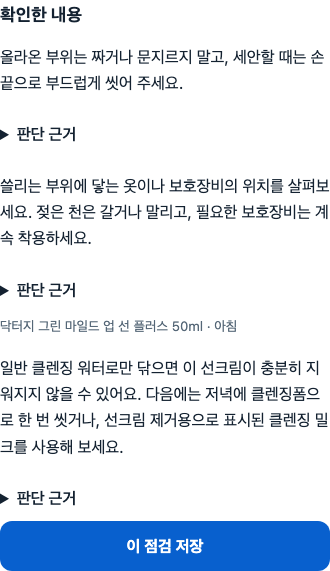
\includegraphics[width=.47\columnwidth,height=48mm,keepaspectratio]{water.png}\hfill
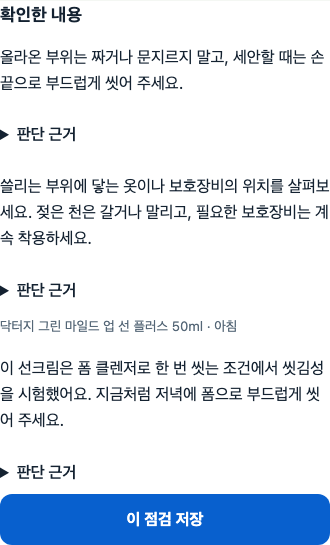
\includegraphics[width=.47\columnwidth,height=48mm,keepaspectratio]{foam.png}
\caption{Synthetic Case 6 development screenshots. Left: water-only answer. Right: foam answer. The same routine is kept in both runs.}
\label{fig:case}
\end{figure}

\subsection{Verification Summary}
The candidate passed 67 frontend checks. The server and data total was 169 after an expiry-boundary regression passed in a separate rerun. The signed device bundle's web assets and catalog matched the tested candidate. The public KB preview has its own verification record, including five discrepancies in the historical 57-case audit. These counts measure software checks and do not establish clinical efficacy. Presentation materials, the demo recording, and physical mirror verification are tracked separately for the E milestone.

\subsection*{Project References}
\begin{itemize}
\item \href{https://github.com/rnehdud/ppopy/tree/main/courses/software-engineering/submissions/phase2/2026-11-06}{Phase 2 Submission B and requirement definitions}
\item \href{https://github.com/rnehdud/ppopy/blob/main/docs/verification.md}{Public preview verification record}
\item \href{https://github.com/rnehdud/ppopy/tree/main/KB/Poppy_KB_v0.6.1/case-6}{Sunscreen-removal Case 6 and supporting evidence}
\end{itemize}
\end{document}
